% !TEX root = ../sethomas_thesis_main.tex

\chapter{Overview of SMA Actuator Design}\label{chap:sma-actuator-design}
\section{Introduction}
In the scope of miniaturisation, creating highly integrated robotic system has become possible with the help of smart materials, notably Shape Memory Alloys (SMA). These alloys, having the highest work density, has made it possible to create miniature artificial muscles that can be integrated into compact and lightweight applications. SMAs have an interesting behaviour which consists of recovery any strain imposed on it when heated above a certain critical temperature threshold, often referred to as the Shape Memory Effect (SME). These alloys exploit the SME to create reversible actuators that are lightweight and compact. This effect is highly non-linear and is dependant on multiple variables, resulting in a highly complex and difficult to model behaviour. Thus, designing and sizing these alloys to create optimised actuators for complex applications is difficult and cumbersome.

In this chapter, an overview of the different implementations of SMA actuators are explored. In the context of different applications, the SMA actuators that are embedded in the different robotic systems are investigated. The traditional design methodology for these actuators are studied and presented in this chapter. The different examples of SMA actuators are used to create a conventional design methodology and the different subsystems of the robotic systems are studied. In this chapter, an in-depth look into the advantages and limitation of the methodology is conducted. In this manner, the conventional design methodology can be adapted into taking a holistic view of the robotic system and create a novel design approach that further promotes the integration of the SMA actuator subsystems into the final robotic system.
% application of sma actuators

\section{Working Principle of SMA Actuators}
Shape Memory Alloys are subclass of smart materials that react to heat. This special brand of material where the can mechanically react with the help of some micro-structural changes when subjected to an external non-mechanical stimulus, in this case, temperature. The shape memory effect that occurs in this alloys occurs due to some phase transformation that happens when heated and cooled around a certain transition temperature. At low temperatures, the material exists in its Martensitic (M) phase where the material can be deformed easily. These deformations, similar to plastic deformation, results in the material being permanently deformed at these low temperatures. As the alloy is heated up its transition temperature, the material transforms from the M phase to the Austenitic (A) phase, recovering any of the \textit{"permanent"} strain imposed on it at low temperatures. This capacity to recover any strain imposed on it and return back to its original shape is often referred to as the shape memory effect. As the material cools below the transition temperature, the alloy returns back to the M phase, allowing the material to be \textit{"plastically"} deformed once again. The detailed description, along with the analytical and numerical models, is detailed in \cref{chap:sma-model}.

The basic idea behind the implementation of the actuator powered by SMAs is to pair the active material with a biasing element. As stated previously, the SMA element requires a deformation at low temperatures to produce any work when heated to its transition temperature. This implies that for the actuator to behave reversibly and create work cycle, a system is required to deform the SMA at low temperature so as to enable the SMA to produce the actuation when heated. A one-directional SMA actuator is also possible where the SMA is stretched and then heated to revert back to its original shape or constrained to generate an increasing stress based on the applied temperature. These actuators can be used for single actuation application such as deployment mechanisms as shown in the work by \todocite (Mohd Jani 2017 Designing SMA linear actuators). However, in this work, the two-directional SMA actuators are explored and studied. These two-directional actuators require a biasing force as the SMA elements can only in one direction. These linear actuators, thus, require some kind of biasing mechanism that can apply a biasing force in the opposite direction. As shown in the work by \todocite (bellouard), the most common mechanisms used to return the SMA back to its neutral position are bias-springs, dead-weights or another SMA element in an antagonistic configuration as shown in \cref{fig:sma-actuators-diagram}.

\begin{figure}[hbt!]
    \centering
    % !TEX root = ../sethomas_thesis_main.tex
\documentclass[border=1mm,
               class=article
               preview]{standalone}
% \usepackage{tikz}
% \usetikzlibrary{decorations.pathmorphing,patterns}
% trim={<left> <lower> <right> <upper>}

\begin{document}
\begin{tikzpicture}[every node/.style={draw,outer sep=0pt,ultra thick,font=\footnotesize}]
\tikzstyle{sma}=[ultra thick,decorate,decoration={zigzag,pre length=4mm,post length=4mm,segment length=4mm, amplitude=2.5mm}]
\tikzstyle{spring}=[ultra thick,decoration={aspect=0.5,pre length=4mm,post length=4mm,segment length=2mm, amplitude=2.5mm,coil},decorate]
\tikzstyle{ground}=[pattern=north east hatch, hatch distance=3mm, hatch thickness=.5pt, fill,draw=none,minimum width=2mm,minimum height=0.1mm]
% \tikzstyle{ground}=[fill,pattern=north east lines,draw=none,minimum width=2mm,minimum height=0.1mm]
% \tikzstyle{damper}=[thick,decoration={markings,
%   mark connection node=dmp,
%   mark=at position 0.5 with
%   {
%     \node (dmp) [thick,inner sep=0pt,transform shape,rotate=-90,minimum width=15pt,minimum height=3pt,draw=none] {};
%     \draw [thick] ($(dmp.north east)+(2pt,0)$) -- (dmp.south east) -- (dmp.south west) -- ($(dmp.north west)+(2pt,0)$);
%     \draw [thick] ($(dmp.north)+(0,-5pt)$) -- ($(dmp.north)+(0,5pt)$);
% }
%   }, decorate]

    % SMA - Spring
    \node (M) [minimum width=20,minimum height=20] {};
    \node (ground) [ground,anchor=north,yshift=-0.25cm,minimum width=1cm] at (M.south) {};
    \draw[ultra thick] (ground.north east) -- (ground.north west);
    \draw [ultra thick] (M.south west) ++ (0.2cm,-0.125cm) circle (0.1cm)  (M.south east) ++ (-0.2cm,-0.125cm) circle (0.1cm);
    \node (groundL) at (M.east) [ground, xshift=-3cm, rotate=-90, minimum height=0.1mm, minimum width=8mm] {};
    \draw[ultra thick] (groundL.north west) -- (groundL.north east);
    \node (groundR) at (M.west) [ground, xshift=+3cm, rotate=90, minimum height=0.1mm, minimum width=8mm] {};
    \draw[ultra thick] (groundR.north west) -- (groundR.north east);
    \draw[spring, color=mygreen] (M.east) -- node[draw=none, anchor=south, yshift=+4mm] {Bias-Spring} (groundR.north);
    \draw[sma, color=myred] (M.west) -- node[draw=none, anchor=south, yshift=+4mm] {SMA} (groundL.north);

    % SMA - SMA
    \begin{scope}[xshift=7cm]
    \node (M) [minimum width=20,minimum height=20] {};
    \node (ground) [ground,anchor=north,yshift=-0.25cm,minimum width=1cm] at (M.south) {};
    \draw[ultra thick] (ground.north east) -- (ground.north west);
    \draw [ultra thick] (M.south west) ++ (0.2cm,-0.125cm) circle (0.1cm)  (M.south east) ++ (-0.2cm,-0.125cm) circle (0.1cm);
    \node (groundL) at (M.east) [ground, xshift=-3cm, rotate=-90, minimum height=0.1mm, minimum width=8mm] {};
    \draw[ultra thick] (groundL.north west) -- (groundL.north east);
    \node (groundR) at (M.west) [ground, xshift=+3cm, rotate=90, minimum height=0.1mm, minimum width=8mm] {};
    \draw[ultra thick] (groundR.north west) -- (groundR.north east);
    \draw[sma, color=mygreen] (M.east) -- node[draw=none, anchor=south, yshift=+4mm] {Antagonist SMA} (groundR.north);% Ant SMA
    \draw[sma, color=myred] (M.west) -- node[draw=none, anchor=south, yshift=+4mm] {SMA} (groundL.north);
    \end{scope}

    % SMA - Deadweight
    \begin{scope}[xshift=3.5cm, yshift=-2cm]
    \node (M) [minimum width=20,minimum height=20] {};
    \node (ground) [ground,anchor=north,yshift=-0.25cm,minimum width=1cm] at (M.south) {};
    \draw[ultra thick] (ground.north east) -- (ground.north west);
    \draw [ultra thick] (M.south west) ++ (0.2cm,-0.125cm) circle (0.1cm)  (M.south east) ++ (-0.2cm,-0.125cm) circle (0.1cm);
    \node (groundL) at (M.east) [ground, xshift=-3cm, rotate=-90, minimum height=0.1mm, minimum width=8mm] {};
    \draw[ultra thick] (groundL.north west) -- (groundL.north east);
    \node (DW) [minimum width=15,minimum height=15, xshift=+2cm, yshift=-1.5cm, color=mygreen] {$m$};
    \node[draw=none, below=1mm of DW.south, color=mygreen] {Deadweight};
    % Pulley
    \node (intermDW) [right=2.5cm of M.east, above=1cm of DW, draw=none] {};
    \draw[ultra thick] ($(intermDW)-(4mm,3mm)$) circle (4mm);
    \draw[ultra thick, rounded corners=4mm, color=mygreen] (M.east) -| (DW.north);
    \draw[ultra thick,fill] ($(intermDW)-(4mm,3mm)$) circle (0.5mm);
    \draw[ultra thick, fill] ($(intermDW)-(4mm,3mm)$) -- ++(2mm,7mm) -- ++(-4mm,0) -- cycle;
    \draw[sma, color=myred] (M.west) -- node[draw=none, anchor=south, yshift=+4mm] {SMA} (groundL.north);
    \end{scope}

    % \draw [sma] (ground1.north) -- ($(M.south east)!(ground1.north)!(M.south west)$);

\end{tikzpicture}
\end{document}

    % \resizebox{0.7\textwidth}{!}{% !TEX root = ../sethomas_thesis_main.tex
\documentclass[border=1mm,
               class=article
               preview]{standalone}
% \usepackage{tikz}
% \usetikzlibrary{decorations.pathmorphing,patterns}
% trim={<left> <lower> <right> <upper>}

\begin{document}
\begin{tikzpicture}[every node/.style={draw,outer sep=0pt,ultra thick,font=\footnotesize}]
\tikzstyle{sma}=[ultra thick,decorate,decoration={zigzag,pre length=4mm,post length=4mm,segment length=4mm, amplitude=2.5mm}]
\tikzstyle{spring}=[ultra thick,decoration={aspect=0.5,pre length=4mm,post length=4mm,segment length=2mm, amplitude=2.5mm,coil},decorate]
\tikzstyle{ground}=[pattern=north east hatch, hatch distance=3mm, hatch thickness=.5pt, fill,draw=none,minimum width=2mm,minimum height=0.1mm]
% \tikzstyle{ground}=[fill,pattern=north east lines,draw=none,minimum width=2mm,minimum height=0.1mm]
% \tikzstyle{damper}=[thick,decoration={markings,
%   mark connection node=dmp,
%   mark=at position 0.5 with
%   {
%     \node (dmp) [thick,inner sep=0pt,transform shape,rotate=-90,minimum width=15pt,minimum height=3pt,draw=none] {};
%     \draw [thick] ($(dmp.north east)+(2pt,0)$) -- (dmp.south east) -- (dmp.south west) -- ($(dmp.north west)+(2pt,0)$);
%     \draw [thick] ($(dmp.north)+(0,-5pt)$) -- ($(dmp.north)+(0,5pt)$);
% }
%   }, decorate]

    % SMA - Spring
    \node (M) [minimum width=20,minimum height=20] {};
    \node (ground) [ground,anchor=north,yshift=-0.25cm,minimum width=1cm] at (M.south) {};
    \draw[ultra thick] (ground.north east) -- (ground.north west);
    \draw [ultra thick] (M.south west) ++ (0.2cm,-0.125cm) circle (0.1cm)  (M.south east) ++ (-0.2cm,-0.125cm) circle (0.1cm);
    \node (groundL) at (M.east) [ground, xshift=-3cm, rotate=-90, minimum height=0.1mm, minimum width=8mm] {};
    \draw[ultra thick] (groundL.north west) -- (groundL.north east);
    \node (groundR) at (M.west) [ground, xshift=+3cm, rotate=90, minimum height=0.1mm, minimum width=8mm] {};
    \draw[ultra thick] (groundR.north west) -- (groundR.north east);
    \draw[spring, color=mygreen] (M.east) -- node[draw=none, anchor=south, yshift=+4mm] {Bias-Spring} (groundR.north);
    \draw[sma, color=myred] (M.west) -- node[draw=none, anchor=south, yshift=+4mm] {SMA} (groundL.north);

    % SMA - SMA
    \begin{scope}[xshift=7cm]
    \node (M) [minimum width=20,minimum height=20] {};
    \node (ground) [ground,anchor=north,yshift=-0.25cm,minimum width=1cm] at (M.south) {};
    \draw[ultra thick] (ground.north east) -- (ground.north west);
    \draw [ultra thick] (M.south west) ++ (0.2cm,-0.125cm) circle (0.1cm)  (M.south east) ++ (-0.2cm,-0.125cm) circle (0.1cm);
    \node (groundL) at (M.east) [ground, xshift=-3cm, rotate=-90, minimum height=0.1mm, minimum width=8mm] {};
    \draw[ultra thick] (groundL.north west) -- (groundL.north east);
    \node (groundR) at (M.west) [ground, xshift=+3cm, rotate=90, minimum height=0.1mm, minimum width=8mm] {};
    \draw[ultra thick] (groundR.north west) -- (groundR.north east);
    \draw[sma, color=mygreen] (M.east) -- node[draw=none, anchor=south, yshift=+4mm] {Antagonist SMA} (groundR.north);% Ant SMA
    \draw[sma, color=myred] (M.west) -- node[draw=none, anchor=south, yshift=+4mm] {SMA} (groundL.north);
    \end{scope}

    % SMA - Deadweight
    \begin{scope}[xshift=3.5cm, yshift=-2cm]
    \node (M) [minimum width=20,minimum height=20] {};
    \node (ground) [ground,anchor=north,yshift=-0.25cm,minimum width=1cm] at (M.south) {};
    \draw[ultra thick] (ground.north east) -- (ground.north west);
    \draw [ultra thick] (M.south west) ++ (0.2cm,-0.125cm) circle (0.1cm)  (M.south east) ++ (-0.2cm,-0.125cm) circle (0.1cm);
    \node (groundL) at (M.east) [ground, xshift=-3cm, rotate=-90, minimum height=0.1mm, minimum width=8mm] {};
    \draw[ultra thick] (groundL.north west) -- (groundL.north east);
    \node (DW) [minimum width=15,minimum height=15, xshift=+2cm, yshift=-1.5cm, color=mygreen] {$m$};
    \node[draw=none, below=1mm of DW.south, color=mygreen] {Deadweight};
    % Pulley
    \node (intermDW) [right=2.5cm of M.east, above=1cm of DW, draw=none] {};
    \draw[ultra thick] ($(intermDW)-(4mm,3mm)$) circle (4mm);
    \draw[ultra thick, rounded corners=4mm, color=mygreen] (M.east) -| (DW.north);
    \draw[ultra thick,fill] ($(intermDW)-(4mm,3mm)$) circle (0.5mm);
    \draw[ultra thick, fill] ($(intermDW)-(4mm,3mm)$) -- ++(2mm,7mm) -- ++(-4mm,0) -- cycle;
    \draw[sma, color=myred] (M.west) -- node[draw=none, anchor=south, yshift=+4mm] {SMA} (groundL.north);
    \end{scope}

    % \draw [sma] (ground1.north) -- ($(M.south east)!(ground1.north)!(M.south west)$);

\end{tikzpicture}
\end{document}
}
    \caption{A schematic representation of the basic types of linear SMA actuators. In general, a separate kinematic stage is used to transform the linear output into the desired output.}
    \label{fig:sma-actuators-diagram}
\end{figure}
The \textbf{Biased-Deadweight SMA Actuator} has the advantage of being quite simple to implement as it consists of simply applying a constant load to the active element irrespective of the temperature. Here, the SMA based on the phase will displace the constant load by a fixed stroke. At low temperatures, the deadweight elongates the SMA element and as the SMA heats up and changes phase, the load will be displaced. As there is always the same constant load, there is a high risk of overheating the SMA and risking reaching stresses above the recommended maximum pull force of the SMA. Thus, to prevent this irreversible damage to the SMA actuator, a constant load that is below the maximum pull force of the SMA is used. This greatly limits the maximum load that can be displaced by the SMA actuator preventing widespread adoption of this method of implementation.

The \textbf{Biased-Spring SMA Actuator}, on the other hand, consists of pairing the SMA element with a biasing passive spring. This method of implementation is also quite simple to implement and thus, is the most widely used method for designing SMA actuators. Here, the idea consists of using a passive spring to apply a spring force to the SMA at low temperatures. This allows the SMA to be deformed and activates the SME when the alloy is heated. As the material transforms from the M to the A phase, the spring is deformed while the SMA element returns to its original shape. Here, due to the increasing elongation of the spring, an increasing spring force acts on the SMA as the temperature is increased. This implies that based on the temperature and the rigidity of the spring, the force and stroke of the actuator can be sized. The sizing methodology and analytical models of this type of actuator will be detailed in \cref{chap:sma-model}. However, the actuator can only be controlled in one direction during the heating phase, while during the cooling, the SMA actuator returns back to its neutral position uncontrolled.


The \textbf{Antagonistic SMA Actuator} consists of pairing the SMA element with an antagonistic biasing SMA element. In this method, the actuator can be actuated in both directions. As the first SMA is heated, the strain recovery cause the antagonistic SMA to be deformed and elongated. When heating the antagonistic SMA, the inverse effect occurs, where the first SMA is deformed and elongated while the antagonistic SMA reverts back to its original shape. Thus, by alternatively heating the SMA pair, the actuator can be made to actuate in both directions. The primary downside to such an implementation is the difficulty in sizing and controlling such an actuator due to the compounding of the highly non-linear nature of each of the SMAs. These SMAs are still widely used in many applications do to the additional degree of freedom. The sizing methodology of these actuators will be described in \cref{chap:sma-model}.

The three methods of implementation represent the majority of the different types of SMA actuators. Using this biasing principle for pre-stretching the SMA element, a reversible and cyclical actuator can be fabricated. It is important to note that the biasing element along with the SMA represent only the subsystems that create the reversible work offered by the active material. However, when creating an SMA actuator, additional structure and elements are required to form a complete actuator for the required application.

\section{Analysis of SMA Actuators}
As stated previously, the principal advantage of actuators powered by SMAs are the fact that, owing to their high work density, these actuators can be designed to be compact and lightweight. However, this is only the case when designed specifically for the required application. Due to the active nature of the material, when the SME is exploited specifically for the requirements of the use case, the resulting actuator can be integrated into the overall robotic application. Thus, when analysing the various methods in which these SMA actuators are designed, it is important to consider the application and its domain. Due to the long cycling time of the SMA elements, SMA actuators are primarily used in systems and domains where low bandwidth but compact actuators are required. Based on the work by \todocite (Mohd Jani, 2014) and \todocite (sreekumar, 2007), these actuators have been used in automotive as miniaturised actuators for various subsystems to replace traditional electromagnetic or pneumatic actuators. In aerospace applications, where there are geometric volume constraints, they have been used to create micro-grippers, vibration dampers or deployment mechanisms. Furthermore, due to their bio-compatibility, these SMA actuators have also found its way into the biomedical field where they have been used to create miniature medical and surgical instruments such as endoscopes, medical tweezers and stents among others. Recently, however, there has been wide interest in creating miniature bio-inspired and reconfigurable robots where these SMAs are used as artificial muscles. Thus, in this section, the goal is to explore the various domains in which SMA actuators are employed and study, using some examples, the different design parameters and choices used to create appropriate actuators for the appropriate application. By doing so, the important and key factors that make up the design of SMA actuators can be established. These factors can, thus, be used to detail the various ares in which these actuators can be improved and optimised such that when designing future SMA actuators, the final systems can be further integrated. By exploring the design choice used in the following examples, a design methodology can be established for creating novel improved SMA actuators.

% Biomedical
\subsection{Biomedical Applications}
Due to the tight volume constraints in the biomedical field, actuators that prioritize compact footprints have been favoured. Furthermore, in the medical field, reduced noise, vibration and contamination are necessary. A high time response is also not required and slower actuation can be tolerated. This makes it an ideal domain for SMA actuators to flourish. The choice of the examples presented in this section is to examine various types of SMA actuators implemented in the biomedical field to extrapolate the various design parameters and choices used for this specific application.
\begin{figure}[hbt!]
    \centering
    % !TEX root = ../../sethomas_thesis_main.tex
\documentclass[border=1mm,
               class=article
               preview]{standalone}
\usepackage{tikz}
% trim={<left> <lower> <right> <upper>}
\begin{document}
\begin{tikzpicture}
    \node[anchor=south west,inner sep=0] (graph) at (0,0) {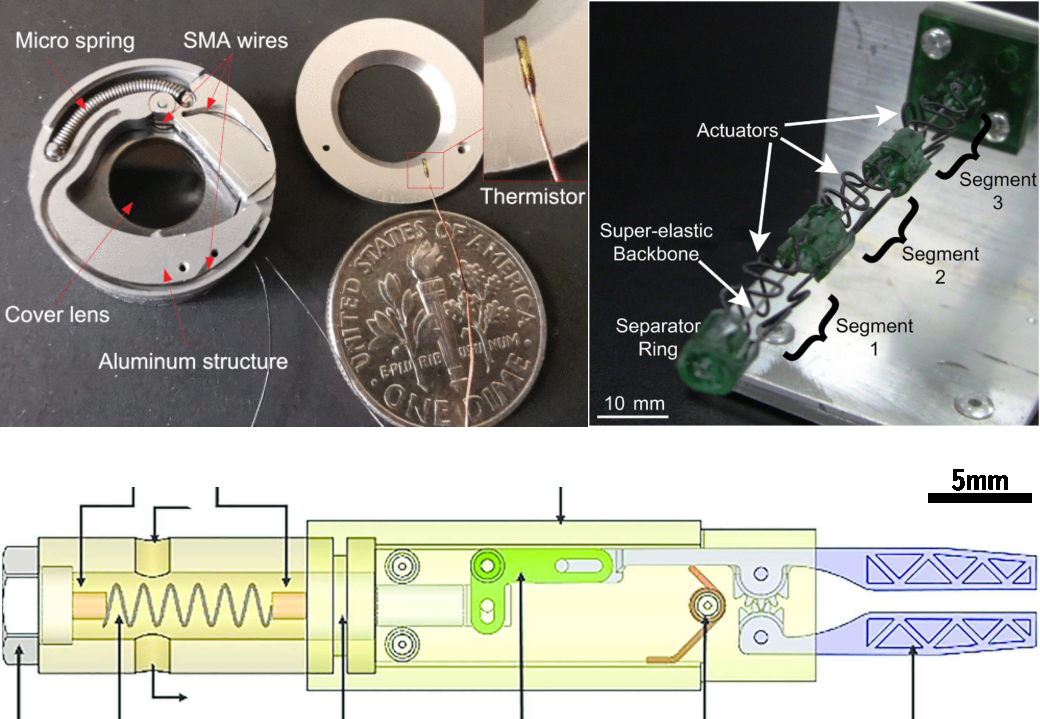
\includegraphics[width=0.7\textwidth]{images/chap1/biomed-examples.pdf}};
    \begin{scope}[x={(graph.south east)},y={(graph.north west)}]
    \node (a) at (0.04,0.46) {\color{white}\textbf{(a)}};
    \node (b) at (0.6,0.95) {\color{white}\textbf{(b)}};
    \node (c) at (0.04,0.37) {\textbf{(c)}};

    \node at (0.02,-0.05) {\footnotesize \makecell[c]{End\\nut}};
    \node at (0.12,-0.05) {\footnotesize \makecell[c]{SMA\\spring}};
    \node at (0.33,-0.02) {\footnotesize Piston};
    \node at (0.5,-0.02) {\footnotesize Link};
    \node at (0.67,-0.05) {\footnotesize \makecell[c]{Steel torsional\\spring}};
    \node at (0.87,-0.05) {\footnotesize \makecell[c]{Gripper\\jaws}};
    \node at (0.17,0.35) {\footnotesize Mount};
    \node at (0.54,0.35) {\footnotesize Base};
    \end{scope}
\end{tikzpicture}
\end{document}

    \caption{An example of an SMA powered actuator used for visual clarity in Surgical cameras taken from the work by \todocite}
    \label{fig:biomed-examples}
\end{figure}

% Automotive / Aerospace
\begin{figure}[hbt!]
    \centering
    % !TEX root = ../../sethomas_thesis_main.tex
\documentclass[border=1mm,
               class=article
               preview]{standalone}
\usepackage{tikz}
% trim={<left> <lower> <right> <upper>}
\begin{document}
\begin{tikzpicture}
    \node[anchor=south west,inner sep=0] (graph) at (0,0) {
        \begin{annotationimage}{trim={0 0cm 0 0cm},clip, width=0.75\textwidth}{images/chap1/auto-examples.pdf}
         \draw[annotation left = {\makecell[r]{SMA\\wire} at 0.7}] to (0.235,0.7);
         \draw[annotation left = {Bias-spring at 0.79}] to (0.24,0.79);
         \draw[annotation left = {Mirror at 0.9}] to (0.1,0.9);
         \draw[annotation right = {\makecell[l]{SMA\\coil} at 0.79}] to (0.74,0.79);
         \draw[annotation right = {\makecell[l]{Power\\electronics} at 0.9}] to (0.7,0.9);
         \draw[annotation right = {Output at 0.7}] to (0.95,0.75);
         \draw[coordinate label = {\color{white}\textbf{(a)} at (0.03,0.96)}];
         \draw[coordinate label = {\color{white}\textbf{(b)} at (0.4,0.96)}];
         \draw[coordinate label = {\color{black}\textbf{(c)} at (0.03,0.56)}];
       \end{annotationimage}};
    % \begin{scope}[x={(graph.south east)},y={(graph.north west)}]
    % \node (a) at (0.14,0.97) {\color{white}\textbf{(a)}};
    % \node (b) at (0.43,0.97) {\color{white}\textbf{(b)}};
    % \node (c) at (0.14,0.56) {\textbf{(c)}};
    % \end{scope}
\end{tikzpicture}
\end{document}

    \caption{An example of an SMA powered actuator used for visual clarity in Surgical cameras taken from the work by \todocite}
    \label{fig:auto-examples}
\end{figure}

% Industrial
\begin{figure}[hbt!]
    \centering
    % !TEX root = ../../sethomas_thesis_main.tex
\documentclass[border=1mm,
               class=article
               preview]{standalone}
\usepackage{tikz}
% trim={<left> <lower> <right> <upper>}
\begin{document}
\begin{tikzpicture}
    \node[anchor=south west,inner sep=0] (graph) at (0,0) {
        \begin{annotationimage}{trim={0 0cm 0 0cm},clip, width=0.9\textwidth}{images/chap1/industrial-examples-v2.pdf}
        % Gripper annotations
        \draw[coordinate label = {\color{black}{\normalfont\tiny{SMA linear actuator}} at (0.565,0.536)}];
        \draw[coordinate label = {\color{black}\normalfont\scriptsize{\makecell[r]{Gripper\\jaw}} at (0.58,0.27)}];
        \draw[coordinate label = {\color{black}\normalfont\scriptsize{\makecell[c]{Cross-shear\\kinematic stage}} at (0.805,0.29)}];
        % Suction annotations
        \draw[coordinate label = {\color{black}\normalfont\scriptsize{Spring adjustment screws} at (0.13,0.525)}];
         \draw[coordinate label = {\color{black}\normalfont\scriptsize{Membrane adjustment} at (0.14,0.47)}];
         \draw[coordinate label = {\color{black}\normalfont\scriptsize{Upper SMA fixation} at (0.16,0.41)}];
         \draw[coordinate label = {\color{black}\normalfont\scriptsize{Bias-spring} at (0.194,0.355)}];
         \draw[coordinate label = {\color{black}\normalfont\scriptsize{SMA wire} at (0.205,0.29)}];
         \draw[coordinate label = {\color{black}\normalfont\scriptsize{Electrical contacts} at (0.165,0.23)}];
         \draw[coordinate label = {\color{black}\normalfont\scriptsize{Lower SMA fixation} at (0.16,0.15)}];

         \draw[coordinate label = {\color{white}\textbf{(a)} at (0.03,0.59)}];
         \draw[coordinate label = {\color{black}\textbf{(b)} at (0.445,0.035)}];
         \draw[coordinate label = {\color{black}\textbf{(c)} at (0.98,0.035)}];
       \end{annotationimage}};
\end{tikzpicture}
\end{document}

    \caption{An example of an SMA powered actuator used for visual clarity in Surgical cameras taken from the work by \todocite}
    \label{fig:industrial-examples}
\end{figure}

% Bio-inspired
\begin{figure}[hbt!]
    \centering
    % !TEX root = ../../sethomas_thesis_main.tex
\documentclass[border=1mm,
               class=article
               preview]{standalone}
\usepackage{tikz}
% trim={<left> <lower> <right> <upper>}

\begin{document}
\begin{tikzpicture}
    \node[anchor=south west,inner sep=0] (graph) at (0,0) {
        \begin{annotationimage}{trim={0 0cm 0 0cm},clip, width=0.9\textwidth}{images/chap1/bio-examples.pdf}
         \draw[coordinate label = {\color{white}\normalfont\tiny{$10$ mm} at (0.68,0.05)}];

         \draw[coordinate label = {\color{black}\textbf{(a)} at (0.03,0.98)}];
         \draw[coordinate label = {\color{black}\textbf{(b)} at (0.98,0.98)}];
         \draw[coordinate label = {\color{white}\textbf{(c)} at (0.27,0.37)}];
       \end{annotationimage}};
      \begin{scope}[x={(graph.south east)},y={(graph.north west)}]
          \node (SMA) at (0.28,0.705) {};
          \node (SMAtext) at (0.28,0.56) {\tiny SMA Coil};
          \draw[latex-] (SMA) -- (SMAtext);
      \end{scope}
\end{tikzpicture}
\end{document}

    \caption{An example of an SMA powered actuator used for visual clarity in Surgical cameras taken from the work by \todocite}
    \label{fig:bio-examples}
\end{figure}

\section{Design Requirements of SMA Actuators}
\section{Traditional SMA Actuator Design}
\subsection{Types of SMA Actuators}
\subsection{Building Blocks of SMA Actuator Design}
\section{Summary and Conclusion}
